%%%%%%%%%%%%%%%%%%%%%%%%%%%%%%%%%%%%%%%%%%%%%%%%%%%%%%%%%%%%%%%%%%
%%%%%%%%%%%%%%%%%%%%%%%%%%%%%%%%%%%%%%%%%%%%%%%%%%%%%%%%%%%%%%%%%%
%Packages
\documentclass[10pt, a4paper]{article}
\usepackage[top=3cm, bottom=4cm, left=3.5cm, right=3.5cm]{geometry}
\usepackage{amsmath,amsthm,amsfonts,amssymb,amscd, fancyhdr, color, comment, graphicx, environ}
\usepackage{float}
\usepackage{subcaption}
\usepackage{mathrsfs}
\usepackage[math-style=ISO]{unicode-math}
\setmathfont{TeX Gyre Termes Math}
\usepackage{lastpage}
\usepackage[dvipsnames]{xcolor}
\usepackage[framemethod=TikZ]{mdframed}
\usepackage{enumerate}
\usepackage[shortlabels]{enumitem}
\usepackage{fancyhdr}
\usepackage{indentfirst}
\usepackage{listings}
\usepackage{sectsty}
\usepackage{thmtools}
\usepackage{shadethm}
\usepackage{hyperref}
\usepackage{setspace}
\usepackage[linguistics]{forest}
\hypersetup{
    colorlinks=true,
    linkcolor=blue,
    filecolor=magenta,      
    urlcolor=blue,
}
%%%%%%%%%%%%%%%%%%%%%%%%%%%%%%%%%%%%%%%%%%%%%%%%%%%%%%%%%%%%%%%%%%
%%%%%%%%%%%%%%%%%%%%%%%%%%%%%%%%%%%%%%%%%%%%%%%%%%%%%%%%%%%%%%%%%%
%Environment setup
\mdfsetup{skipabove=\topskip,skipbelow=\topskip}
\newrobustcmd\ExampleText{%
An \textit{inhomogeneous linear} differential equation has the form
\begin{align}
L[v ] = f,
\end{align}
where $L$ is a linear differential operator, $v$ is the dependent
variable, and $f$ is a given non−zero function of the independent
variables alone.
}
\mdfdefinestyle{theoremstyle}{%
linecolor=black,linewidth=1pt,%
frametitlerule=true,%
frametitlebackgroundcolor=gray!20,
innertopmargin=\topskip,
}
\mdtheorem[style=theoremstyle]{Problem}{Problem}
\newenvironment{Solution}{\textbf{Solution.}}

\definecolor{codegreen}{rgb}{0,0.6,0}
\definecolor{codegray}{rgb}{0.5,0.5,0.5}
\definecolor{codepurple}{rgb}{0.58,0,0.82}
\definecolor{backcolour}{rgb}{0.95,0.95,0.92}

\lstdefinestyle{mystyle}{
    backgroundcolor=\color{backcolour},   
    commentstyle=\color{codegreen},
    keywordstyle=\color{magenta},
    numberstyle=\tiny\color{codegray},
    stringstyle=\color{codepurple},
    basicstyle=\ttfamily\footnotesize,
    breakatwhitespace=false,         
    breaklines=true,                 
    captionpos=b,                    
    keepspaces=true,                 
    numbers=left,                    
    numbersep=5pt,                  
    showspaces=false,                
    showstringspaces=false,
    showtabs=false,                  
    tabsize=2
}

\lstset{style=mystyle}
%%%%%%%%%%%%%%%%%%%%%%%%%%%%%%%%%%%%%%%%%%%%%%%%%%%%%%%%%%%%%%%%%%
%%%%%%%%%%%%%%%%%%%%%%%%%%%%%%%%%%%%%%%%%%%%%%%%%%%%%%%%%%%%%%%%%%
%Fill in the appropriate information below
\newcommand{\norm}[1]{\left\lVert#1\right\rVert}     
\newcommand\course{Data Science}                            % <-- course name     
\newcommand\Information{02451305}                        % <-- personal information
%%%%%%%%%%%%%%%%%%%%%%%%%%%%%%%%%%%%%%%%%%%%%%%%%%%%%%%%%%%%%%%%%%
%%%%%%%%%%%%%%%%%%%%%%%%%%%%%%%%%%%%%%%%%%%%%%%%%%%%%%%%%%%%%%%%%%
%Page setup
\pagestyle{fancy}
\headheight 35pt
\lhead{\today}
\rhead{
\includegraphics[width=2.5cm]{Data/Figure_for_report/icl_logo.png}}
\lfoot{}
\pagenumbering{arabic}
\cfoot{\small\thepage}
\rfoot{}
\headsep 1.2em
\renewcommand{\baselinestretch}{1.25}
%%%%%%%%%%%%%%%%%%%%%%%%%%%%%%%%%%%%%%%%%%%%%%%%%%%%%%%%%%%%%%%%%%
%%%%%%%%%%%%%%%%%%%%%%%%%%%%%%%%%%%%%%%%%%%%%%%%%%%%%%%%%%%%%%%%%%
%Add new commands here
\renewcommand{\labelenumi}{\alph{enumi})}
\newcommand{\Z}{\mathbb Z}
\newcommand{\R}{\mathbb R}
\newcommand{\Q}{\mathbb Q}
\newcommand{\NN}{\mathbb N}
\newcommand{\PP}{\mathbb P}
\DeclareMathOperator{\Mod}{Mod} 
\renewcommand\lstlistingname{Algorithm}
\renewcommand\lstlistlistingname{Algorithms}
\def\lstlistingautorefname{Alg.}
\newtheorem*{theorem}{Theorem}
\newtheorem*{lemma}{Lemma}
\newtheorem{case}{Case}
\newcommand{\assign}{:=}
\newcommand{\infixiff}{\text{ iff }}
\newcommand{\nobracket}{}
\newcommand{\backassign}{=:}
\newcommand{\tmmathbf}[1]{\ensuremath{\boldsymbol{#1}}}
\newcommand{\tmop}[1]{\ensuremath{\operatorname{#1}}}
\newcommand{\tmtextbf}[1]{\text{{\bfseries{#1}}}}
\newcommand{\tmtextit}[1]{\text{{\itshape{#1}}}}

\newenvironment{itemizedot}{\begin{itemize} \renewcommand{\labelitemi}{$\bullet$}\renewcommand{\labelitemii}{$\bullet$}\renewcommand{\labelitemiii}{$\bullet$}\renewcommand{\labelitemiv}{$\bullet$}}{\end{itemize}}
\catcode`\<=\active \def<{
\fontencoding{T1}\selectfont\symbol{60}\fontencoding{\encodingdefault}}
\catcode`\>=\active \def>{
\fontencoding{T1}\selectfont\symbol{62}\fontencoding{\encodingdefault}}
\catcode`\<=\active \def<{
\fontencoding{T1}\selectfont\symbol{60}\fontencoding{\encodingdefault}}




\begin{document}

\begin{titlepage}
    \begin{center}
        \vspace*{3cm}
            
        \Huge
        \textbf{Analysis of middle and long distance running in World Athletics}
            
        \vspace{1cm}
        \huge
            
        \vspace{1.5cm}
        \Large
            
        \textbf{02451305}                      % <-- author
        
            
        \vfill
        
        \course
            
        \vspace{1cm}
            
        
\includegraphics[width=0.4\textwidth]{Data/Figure_for_report/Word_athletic_logo.png}
        \\
        
        \Large
        
        \today
            
    \end{center}
\end{titlepage}


\newpage

I, 02451305, certify that this assessed coursework is my own work, unless otherwise acknowledged, and includes no
plagiarism. I have not discussed my coursework with anyone else except when seeking clarification with the module
lecturer via email or on MS Teams. I have not shared any code underlying my coursework with anyone else prior to
submission.

\newpage

\section*{Introduction}

A few years ago, the "Breaking 2" project, organised by Nike and INEOS around the Kenyan athlete Eliud Kipchoge made the headlines, as he managed to break the symbolic 2 hours barrier for the Marathon. It was as much of a physical prowess than a marketting one for those companies, that allowed Nike to introduce what is presented as a "revolution" for running with their new carbon plated shoes. 
This event brought the headlight on what has been a fast growing sport in recent years. The idea behind this project will be to collect data around the best athlete's performances to have an overview of these athletes who make the sport.

\section{Collecting the data : Web scraping}

NB : All the data collected is available on the World Athletics website. It is technically forbidden by the Terms and conditions of the website to create a database with the data of the website, but the data collected further is public data, free of copyright and doesn't require an account to access. The data collected has no commercial purposes so the European legislation as well as the American one accepts this use of the data (no Terms and Conditions were actively approved ).

\subsection*{Creating the athletes database}

The first step of getting the data was to create the relevant databases of athletes, using the Wold Athletics website (World athletics is the governing body of the professional athletics events). The database (and every analysis to come after) will be split in two distinct parts : one for the men and another one for the women.
To do that, I used the the World rankings as of May 2024 and got the Top 400 athletes in each middle and long distance event : from the 1500m to the Marathon. Keep in mind that one athlete can appear in all of the rankings. In this step I gathered all the basic information about athletes : their name, date of birth, the country they represent and most importantly the URL to their individual profile containing their lifetime performances on a page similar to \ref{fig:athl-scrap}. This database needs little to no processing to be readable.

\begin{figure}
    \centering
    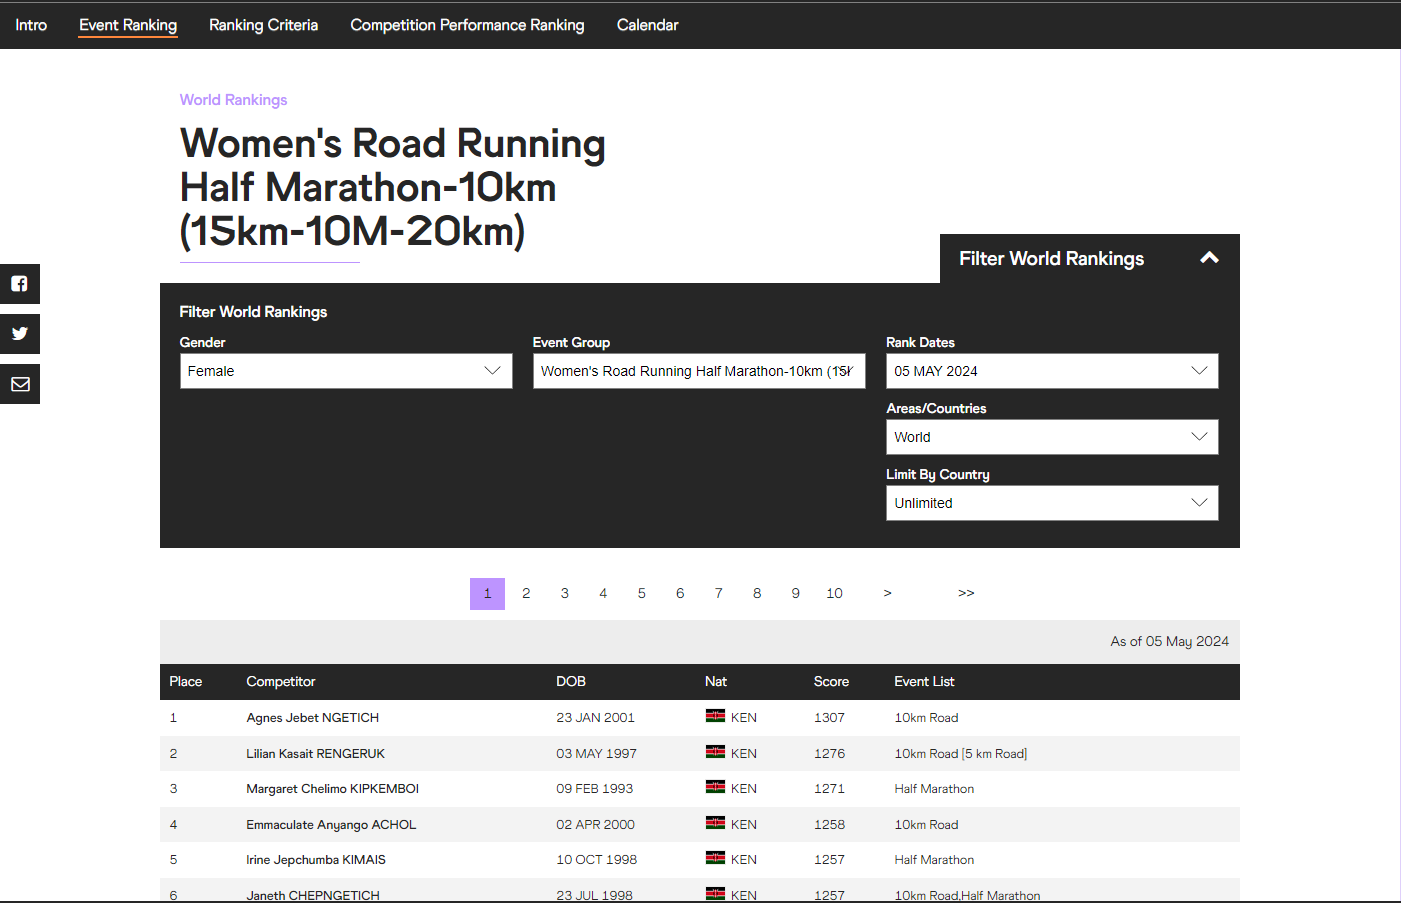
\includegraphics[width=0.5\linewidth]{Data/Figure_for_report/Athlete Scraping.png}
    \caption{Example of a page for athletes information}
    \label{fig:athl-scrap}
\end{figure}

\subsection*{Creating the performance database}

Once I got the full database of athletes, I accessed each individual URL to get for every athlete, the performances in the "Progression" tab on the page. This allowed me to get for every every event their best performance time-wise for each year of competing in World Athletics. At this point, the data gathered is as raw as it can get as the idea was to limit the time spent on a page (it already took around 2 hours to gather all the information). 
It is made of a column with the name of the athlete, and another that contains a array (that is converted into a string in the dataframe) in which are all the information on every athletes 

\begin{figure}
    \centering
    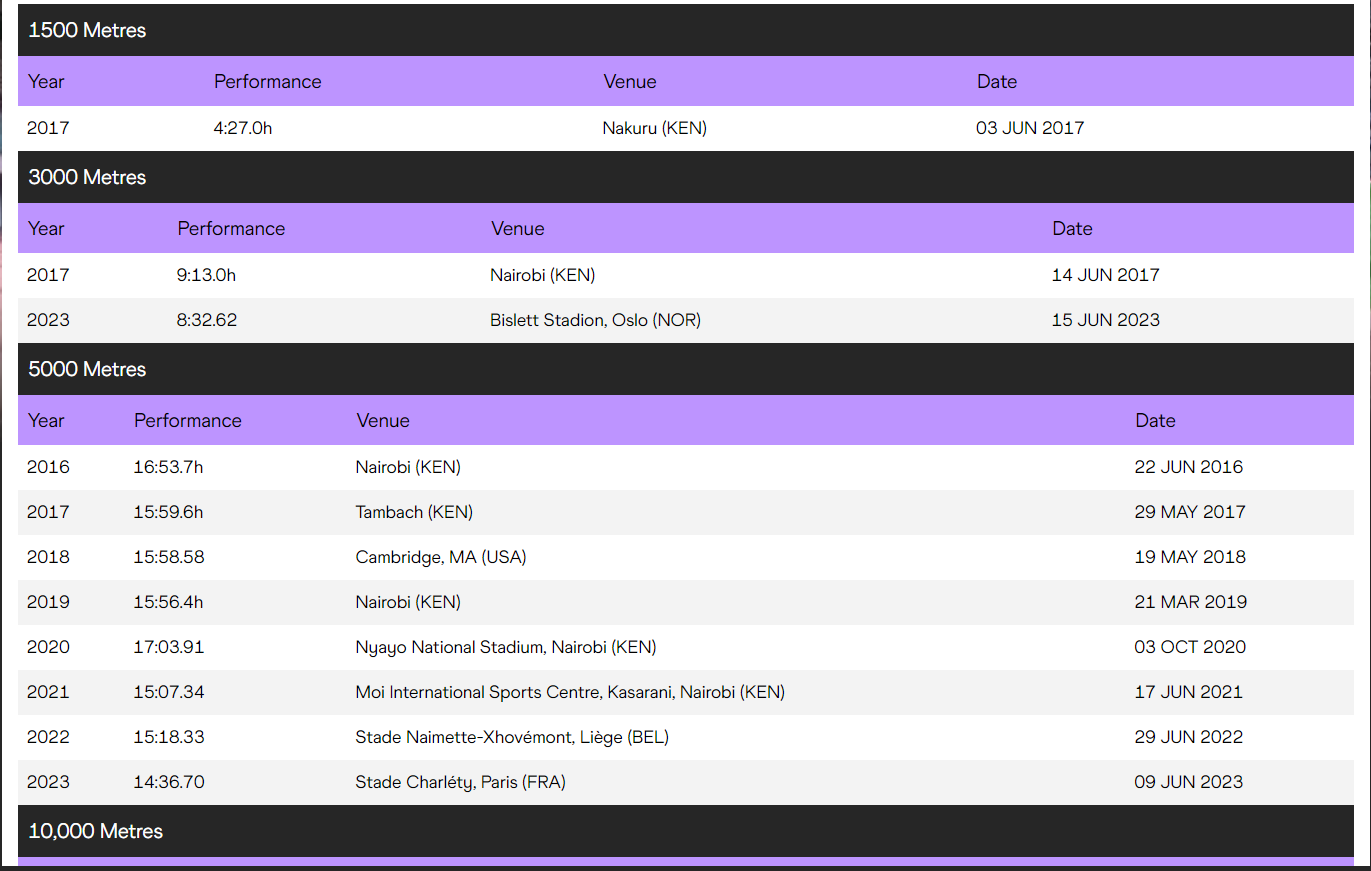
\includegraphics[width=0.5\linewidth]{Data/Figure_for_report/Performance scaping.png}
    \caption{Example of a page for athletes performances}
    \label{fig:perf-scrap}
\end{figure}

\newpage

\section{Preprocessing}

As mentioned before, the rawness of the data especially in the second database requires quite a heavy processing. The athletes databases will remain more or less untouched as only the urls will be filtered out and I will only keep an athlete year of birth compared to their full date of birth. Each line of the performance database will include the athlete's name and the information about a single event they participated in : the race distance, the time achieved and the year the performance was done.

First of all, I am going the filter out all of what we can consider secondary events an athlete takes part in: in the final database will only appear the following events  : 1500m, 5000m track, 10000m track, 5km road, 10 km road, Half Marathon and Marathon. 

To do that I had to split the raw text data that made the races column. Each element in the array was all the information about the performance in the athlete's career in a single distance. Each row of the dataframe will be made of the name of the athlete, a year they raced in, and for all the races considered in this project their best time that year. If they have not raced in a specific distance that year, the value will be NaN. The race times will be loaded as datetimes type so that the Dataframe is easily readable.

Extra processing will be needed depending on the use of the data for the data analysis part but as it stands the dataframe can be used and understood easily.


\newpage

\section{Data analysis}

\subsection{Athletes nationality}

Let's first start with an exploratory analysis of the athletes data, looking at where they come from in the world. For this purpose and this one only, the men and women databases will be be combined, the number of athletes coming from each country were counted. 

\begin{figure}[htb]
    \centering
    \begin{subfigure}[b]{0.45\linewidth}
        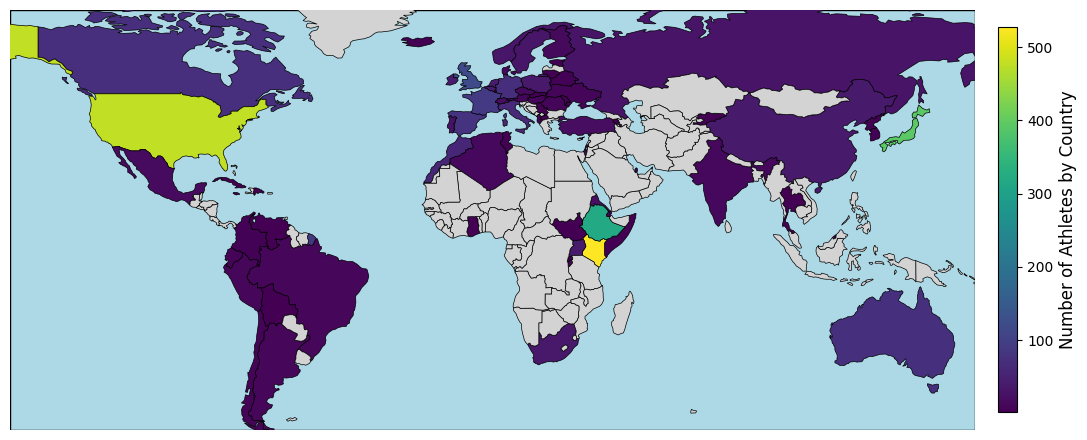
\includegraphics[width=\linewidth]{Data/Figures/Athletes_countries.png}
        \caption{Number of elite athletes per country}
        \label{fig:athletes_country}
    \end{subfigure}
    \hfill
    \begin{subfigure}[b]{0.45\linewidth}
        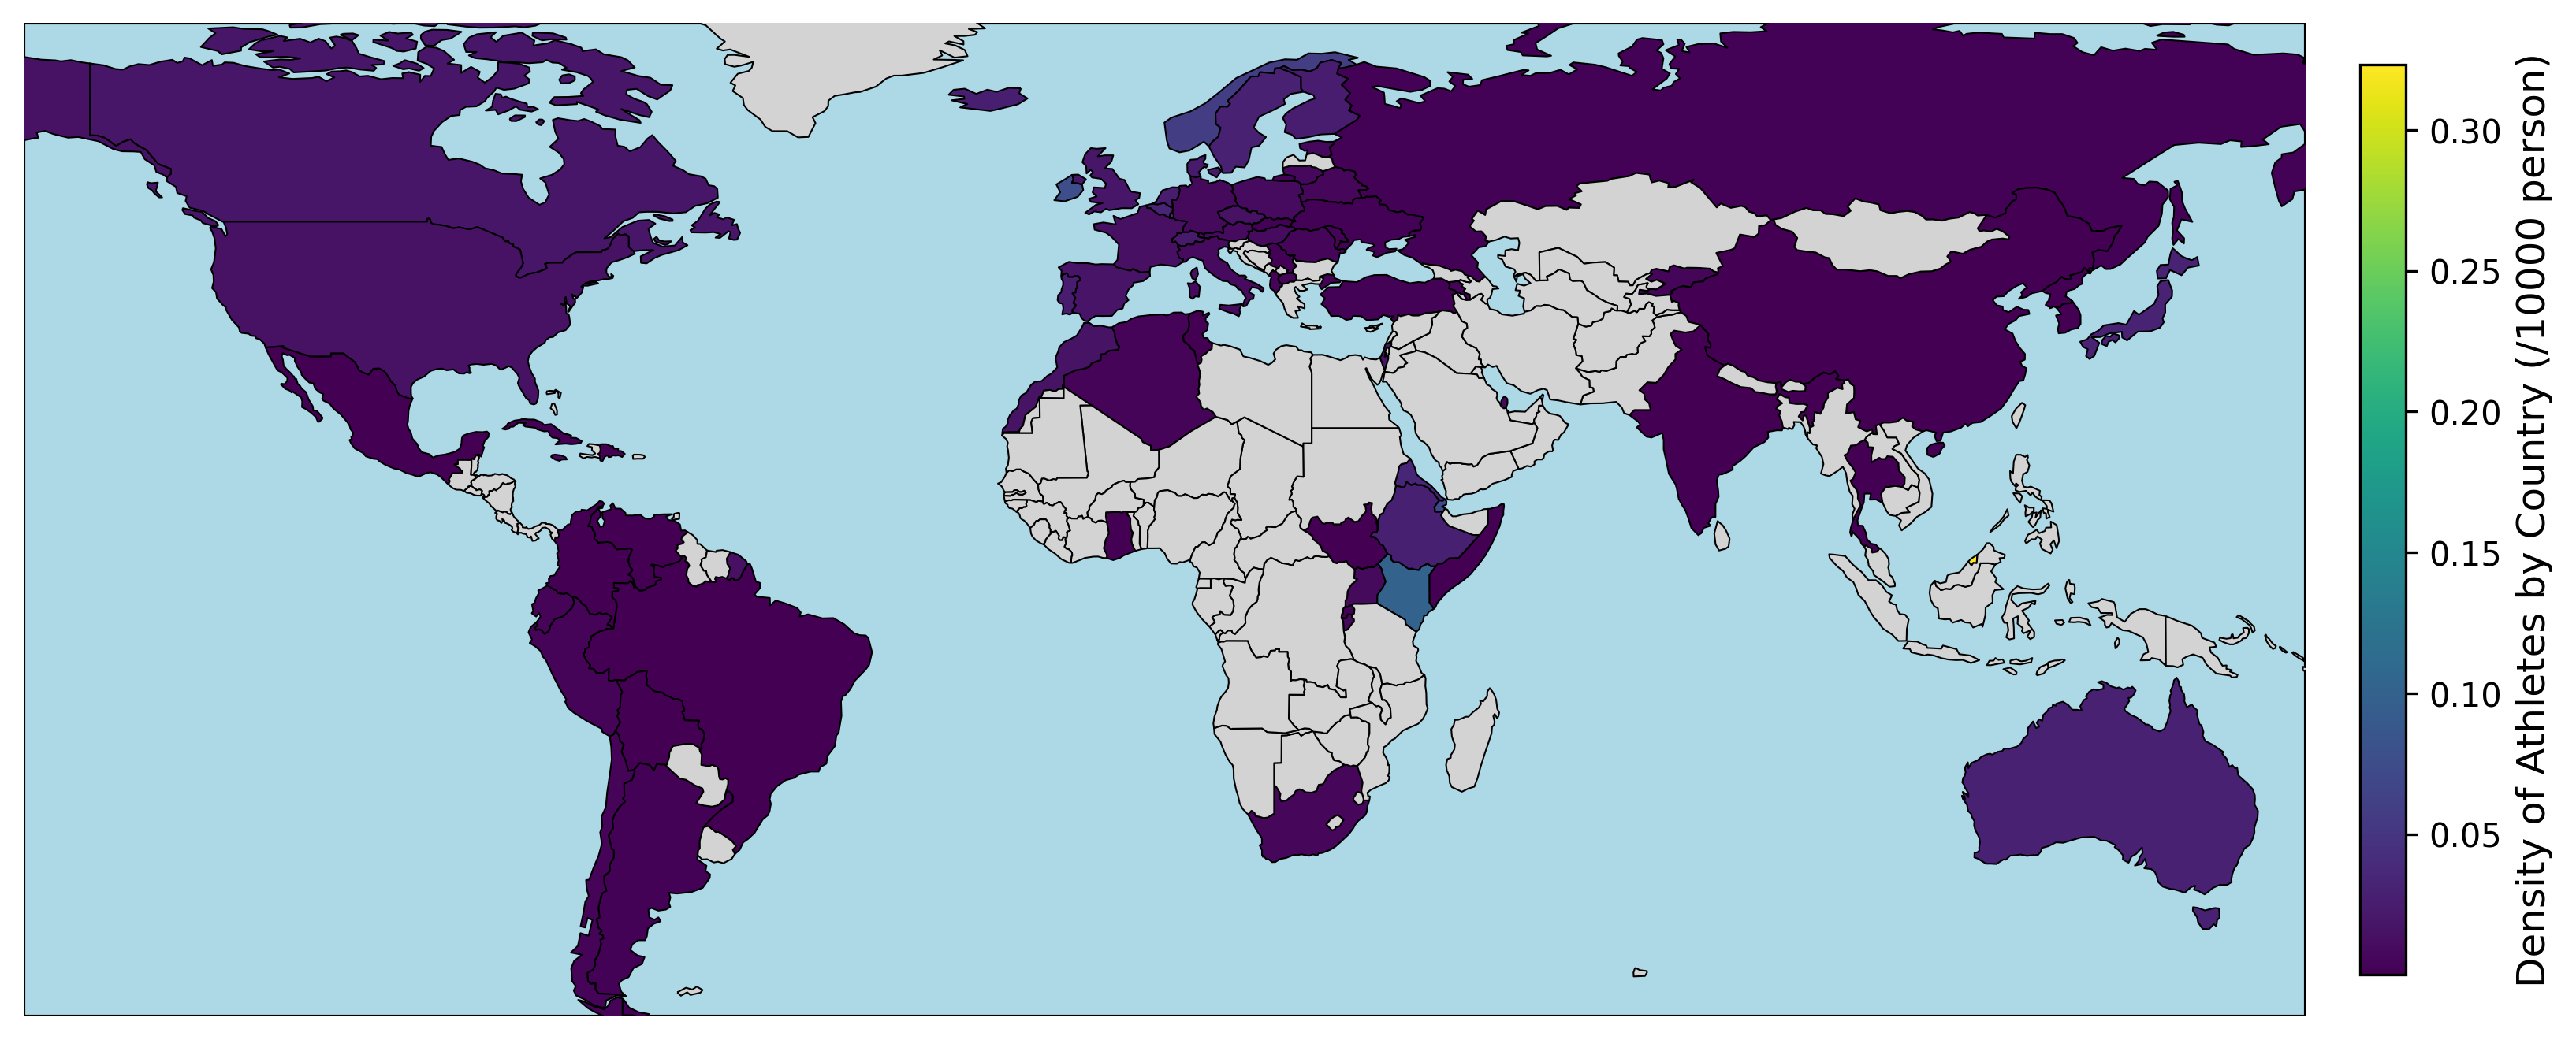
\includegraphics[width=\linewidth]{Data/Figures/Athletes_countries_pop.png}
        \caption{Number of athletes /1000 citizens}
        \label{fig:athletes_pop}
    \end{subfigure}
    \caption{Distribution of athletes per country}
    \label{fig:athletes_countries}
\end{figure}

As we can see in \ref{fig:athletes_countries}, in terms of the sheer number of athletes, two countries from the horn of Africa, Kenya and Ethiopia dominate the contingent of professional athletes. This translates at the highest level of the sport as these athletes are the ones who claim most of the top spots in international competitions (keeping in mind that most of the athletes from those countries often don't have the funding to turn professional, so the ones we see are just the tip of the iceberg). On the other countries like Japan or the United States, look dominant on the professional scene, mostly because of the size of their population. It looks like the rest of the countries are spread out mostly in developed countries, and that the Middle East and Africa (apart from the remarkable exception of Kenya and Ethiopia) are left out of the equation.\\

\subsection{Age distribution}

We are now going to be interested on when these athletes race. This is quite an interesting thing to look at, as the stereotypical path for an elite runner is to start with shorter distance (between 1500 m and 5000m), usually on the track, to evolve towards longer distances like the marathon. The most striking example of such a carreer is Eliud Kipchoge who won 2 Olympic medals and 1 World Champshionship in the 5000m between 2004 and 2010 before transitioning to the most iconic distance in running. He then went on to be one of the best long distance runner in history. 

The following figures \ref{fig:athletes_age} where done by counting the number of athletes who took part in a certain race distance at the relevant age (the number of races or the time they hit didn't take part in here), for each gender. The age variable was treated as a discrete variable, simply using $\text{Age} = \text{Year}_{\text{race}} - \text{Year}_{\text{birth}}$.


\begin{figure}[htb]
    \centering
    \begin{subfigure}[b]{0.45\linewidth}
        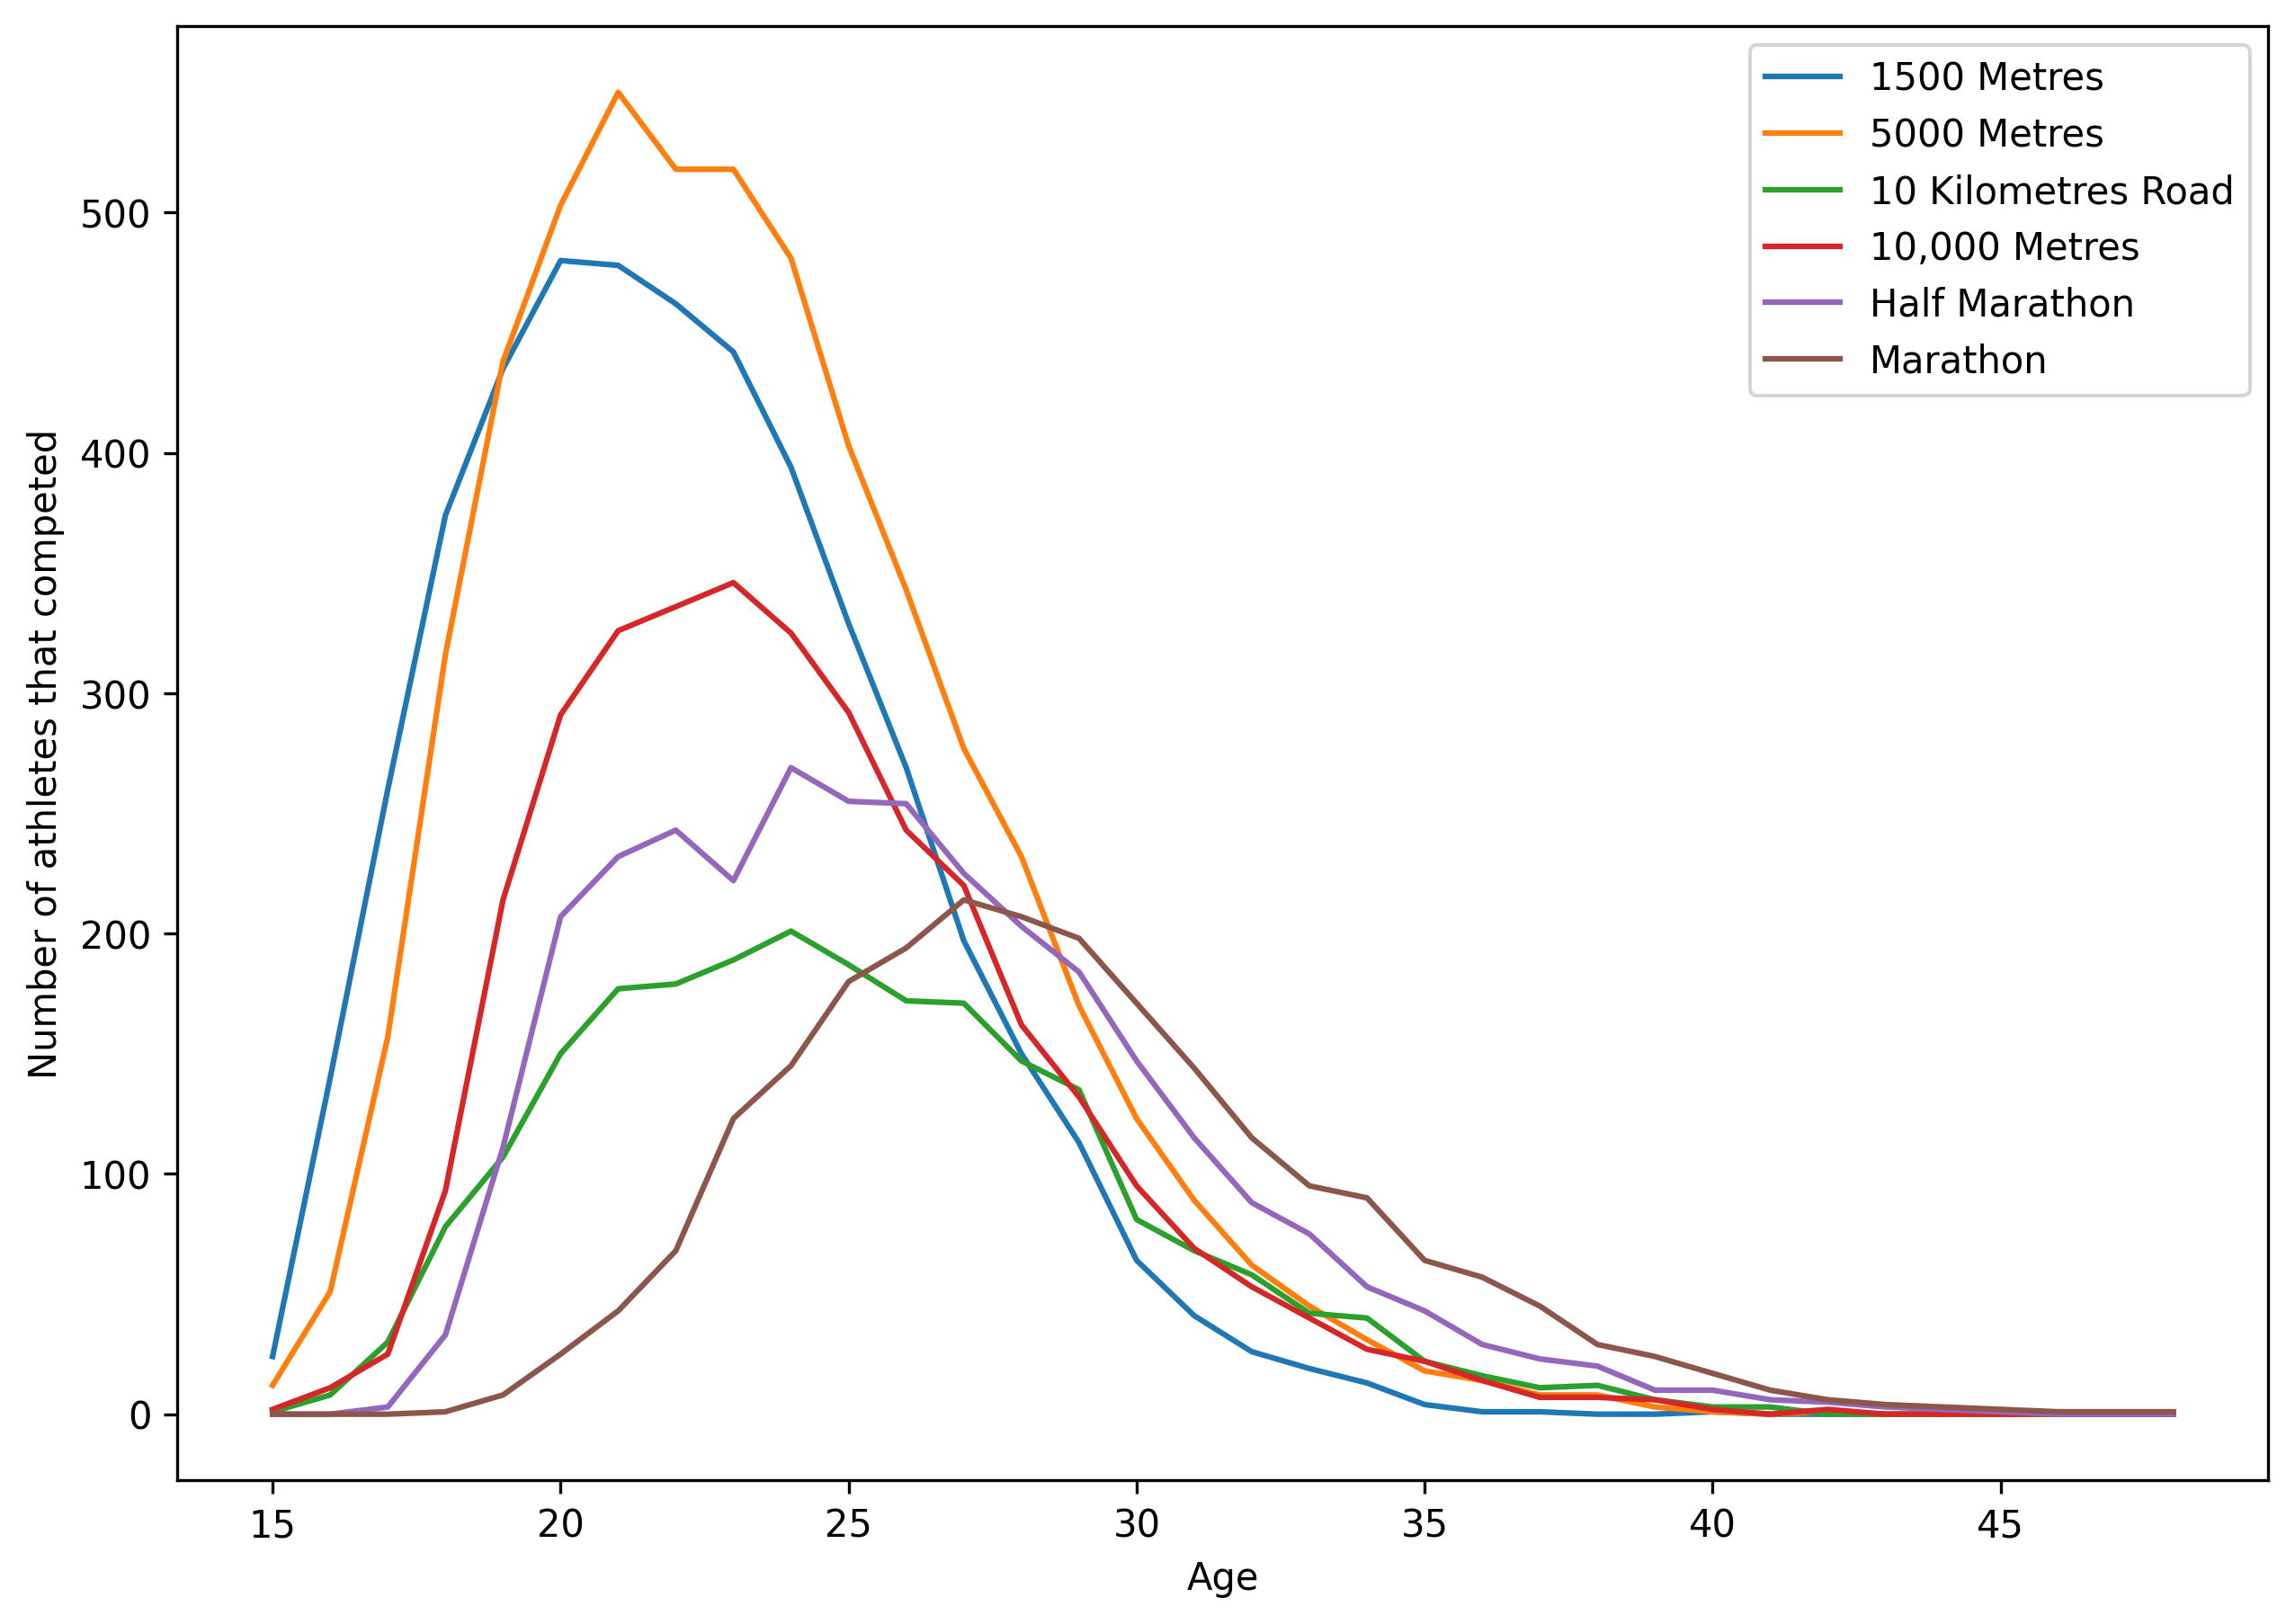
\includegraphics[width=\linewidth]{Data/Figures/Men_Athletes_distribution.png}
        \caption{Average age for men}
        \label{fig:men_age}
    \end{subfigure}
    \hfill
    \begin{subfigure}[b]{0.45\linewidth}
        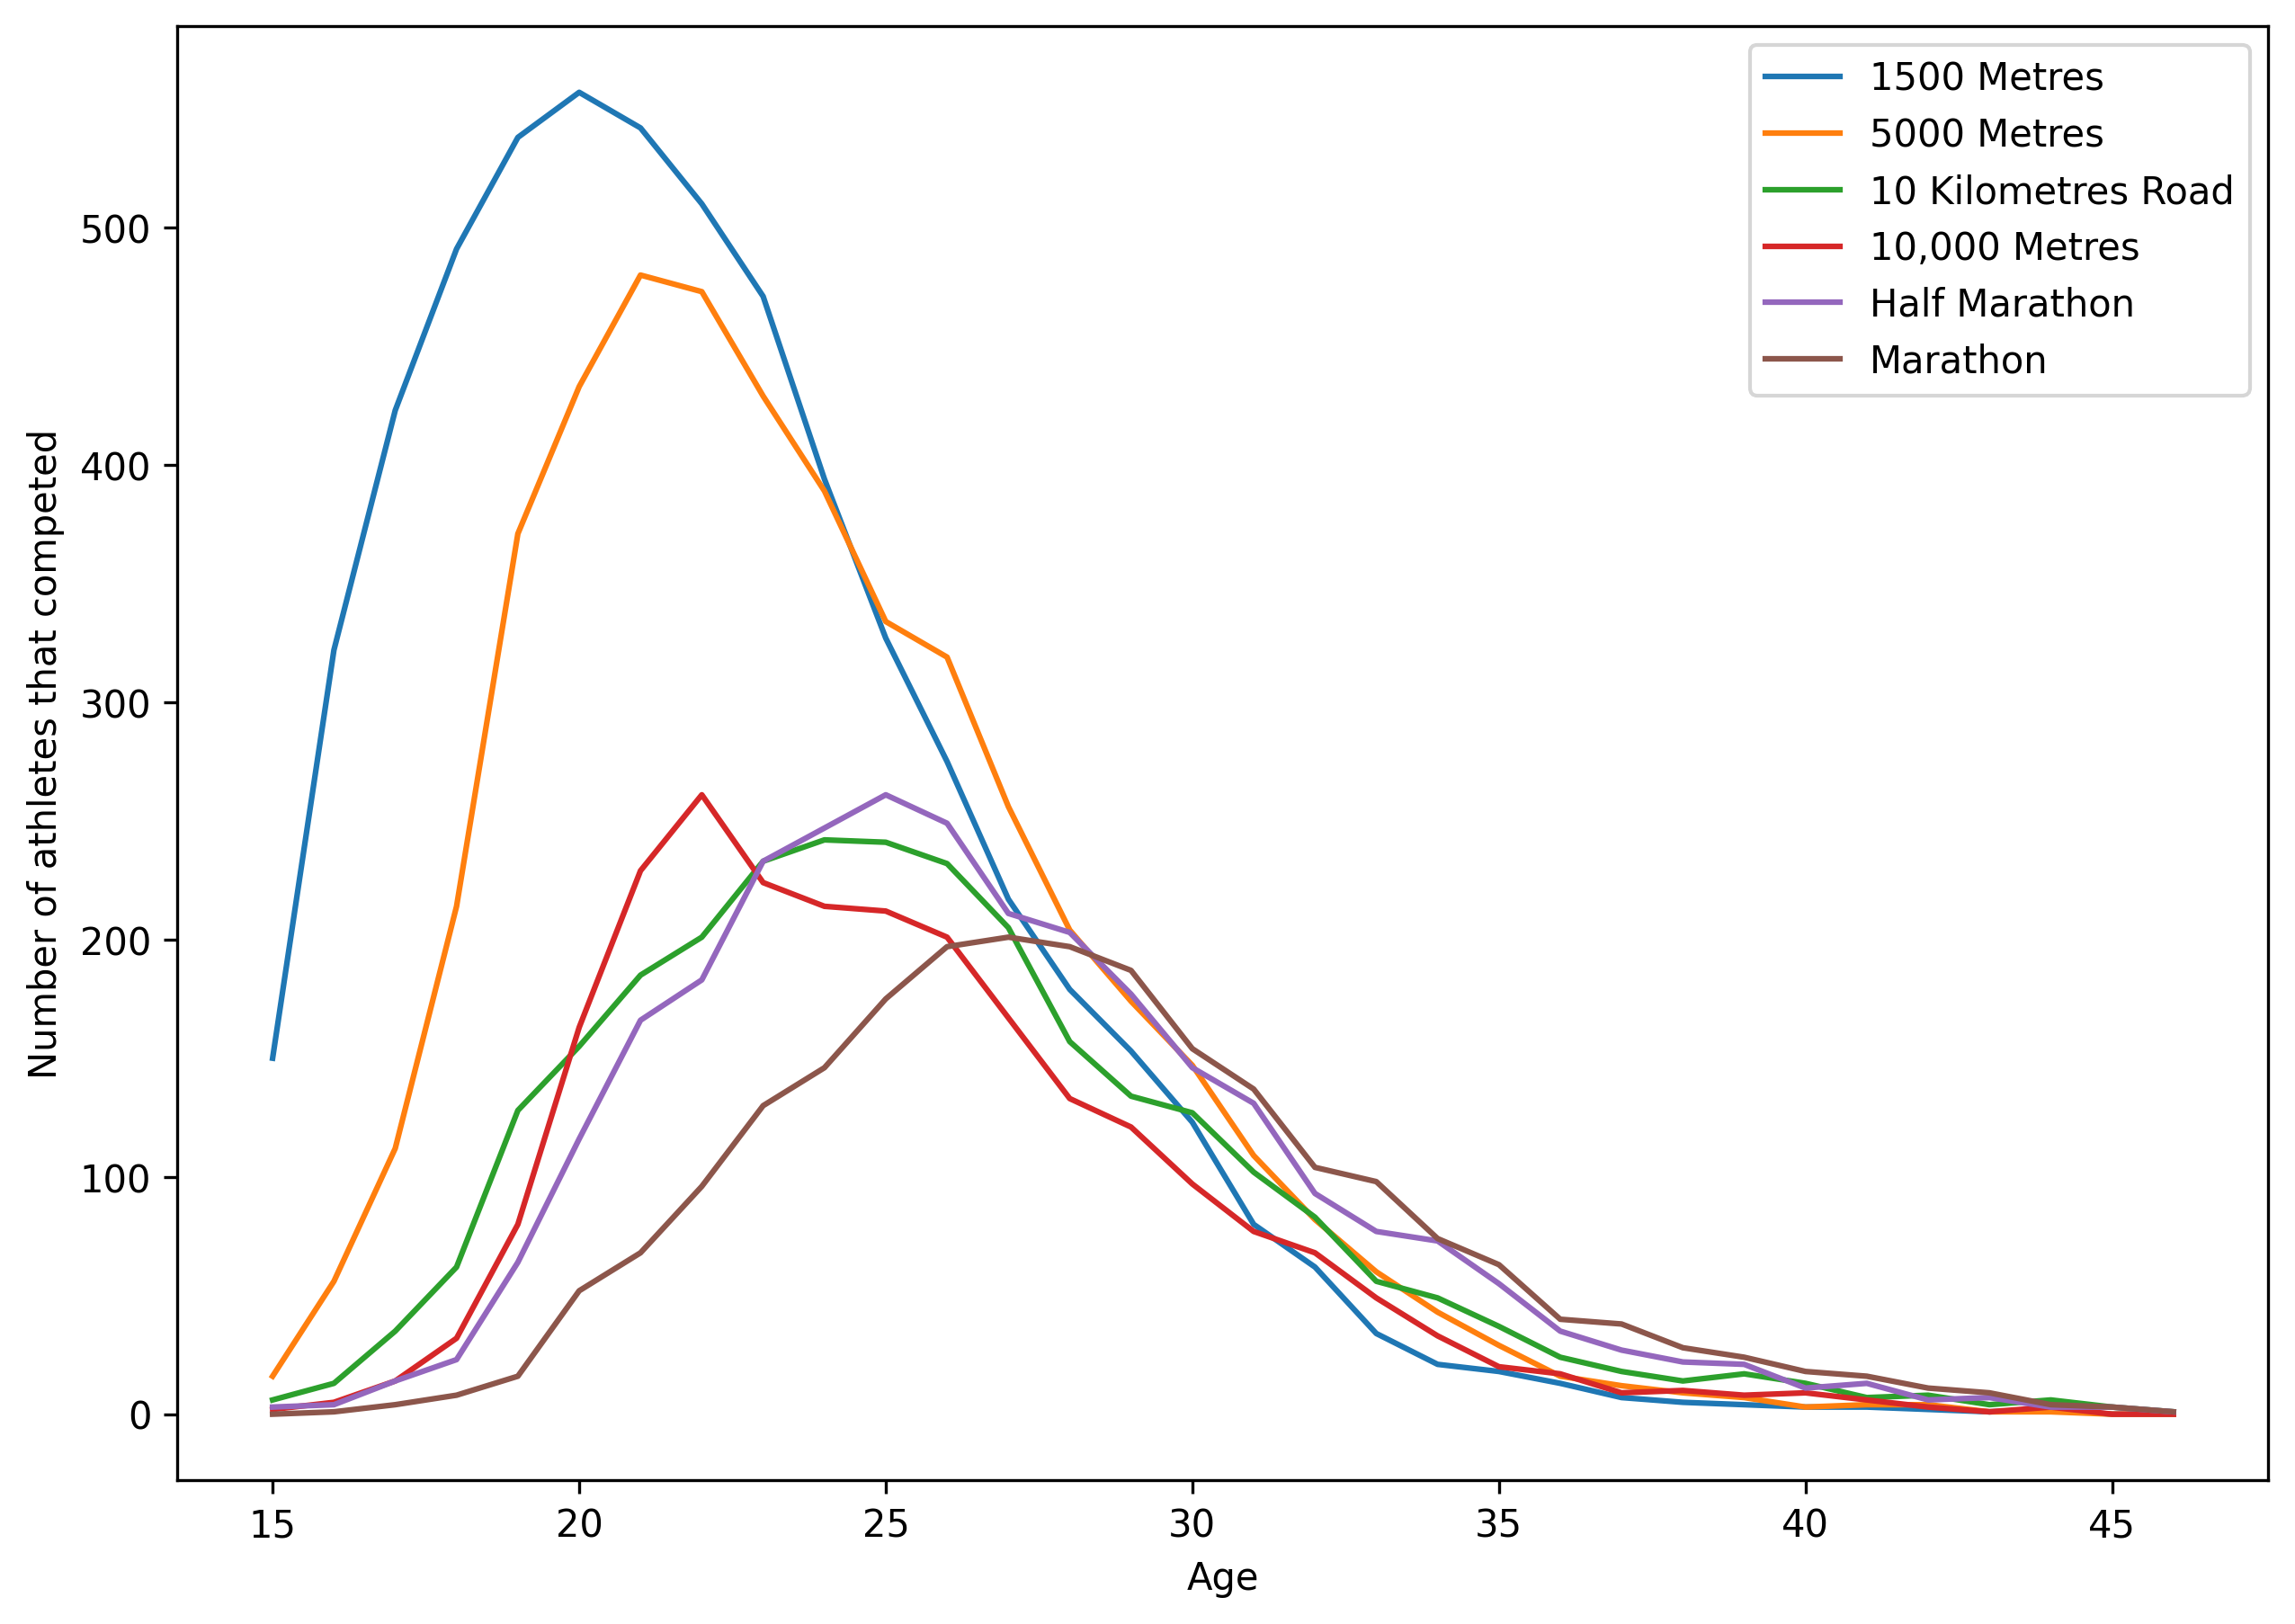
\includegraphics[width=\linewidth]{Data/Figures/Women_Athletes_distribution.png}
        \caption{Average age for women}
        \label{fig:women_age}
    \end{subfigure}
    \caption{Distribution of athletes per age}
    \label{fig:athletes_age}
\end{figure}

Both figures \ref{fig:athletes_age} illustrate this typical career path : we could assume the distributions to be Poisson with $\lambda>1$ and evidently, the longer the distance, the bigger the $\lambda$. Interestingly enough, male athletes seem to transition slower to long distances than female athletes where the 10000m is a lot less popular among them. Apart from that both the men and women have the same trajectory in their career. \\


\subsection{Average progression}

Going further than just looking at when they race, I am going to look at the evolution of their personal best during their career.

The first step is creating a personal best column for each distance the athlete raced in during his life. This is done by first sorting the values in the dataframe by athlete and year. With the newly sorted dataframe, the idea is to group by name in the dataframe and apply a function that computes the rolling minimum (saying that a lower time finish equates to a better performances), which we denote by Rmin for a list A, $i \in \mathbf{N}$ and $ i\leq \text{len}(A)$ : $$\text{Rmin}(A,i) = \text{min}((A_j)_{j\leq i}) = \text{min}(\text{Rmin}(A,i-1),i)$$, using the convention that $\text{min}(\text{NaN},i) = i$ for any $i$. Using this, we get for each athlete a dataframe with decreasing columns containing their best time in seconds up until that year (with NaN values for every year before their first race in that distance).

Using this newly created dataframe, all we need to do is still grouping by the name of the athlete, compute the difference of their personal best between two consecutive years, with the rule that a progression is non-negative for readability purposes. Because of the increasing nature of the sequences, this difference will either be 0 or positive (or NaN). This difference was scaled using typical times for every distance (as an example for men, the scale was 3:40 for 1500m, 14:00 for 5000m, 29:00 for 10km, 61:00 for the half marathon and 2:06 for the full Marathon) to compare the time improvement between different events. The scaling was obviously different for women, as we typically notice a $10\%$ difference between male and female performances, over all distances so this translates in the scales used.

Once we have gotten that, what is left is averaging the values over every athlete, for a given age. Once again, the mean function used will ignore the NaN values to give a mean of the existing values. We get the evolution of the average progression for athlete over different distances in figure \ref{fig:athletes_progression}. The window was chosen to make sure the focus was on the range that matches with the peak of the athletes, because the data was too sparse before the age of 20 and after 35 to have significant results.

\begin{figure}[htb]
    \centering
    \begin{subfigure}[b]{0.45\linewidth}
        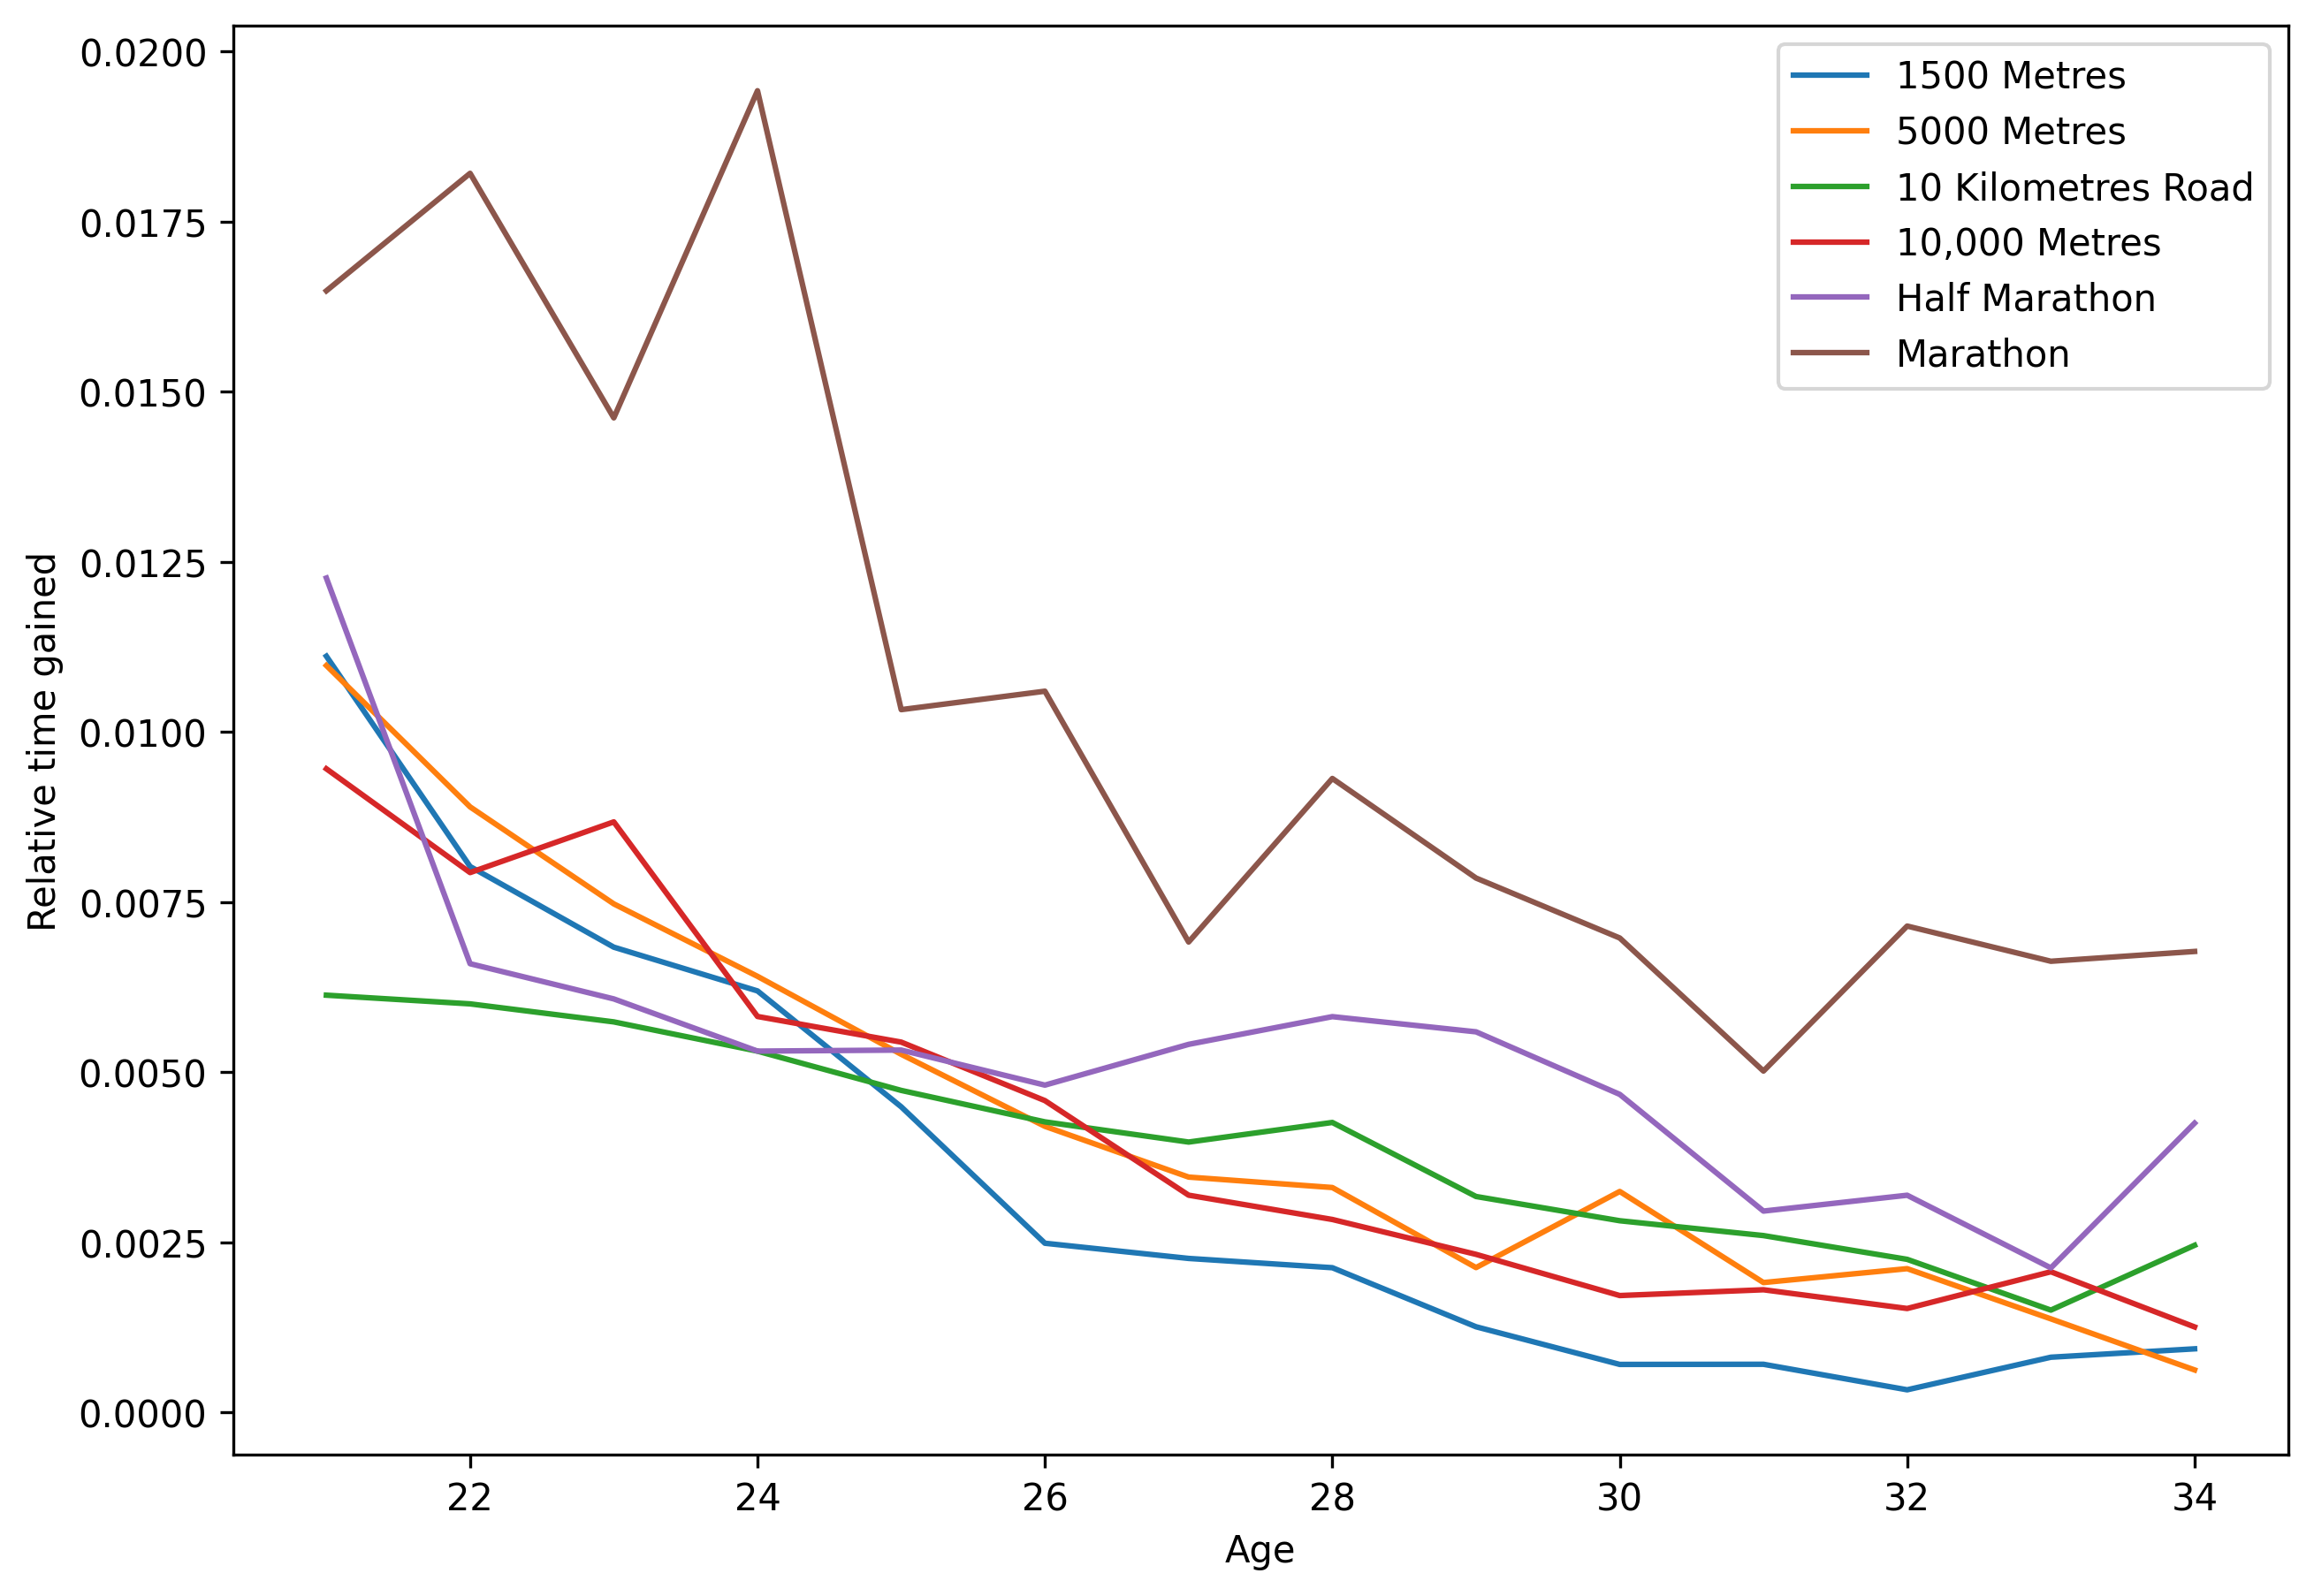
\includegraphics[width=\linewidth]{Data/Figures/Men_Athletes_progression.png}
        \caption{Average progression for men}
        \label{fig:men_progression}
    \end{subfigure}
    \hfill
    \begin{subfigure}[b]{0.45\linewidth}
        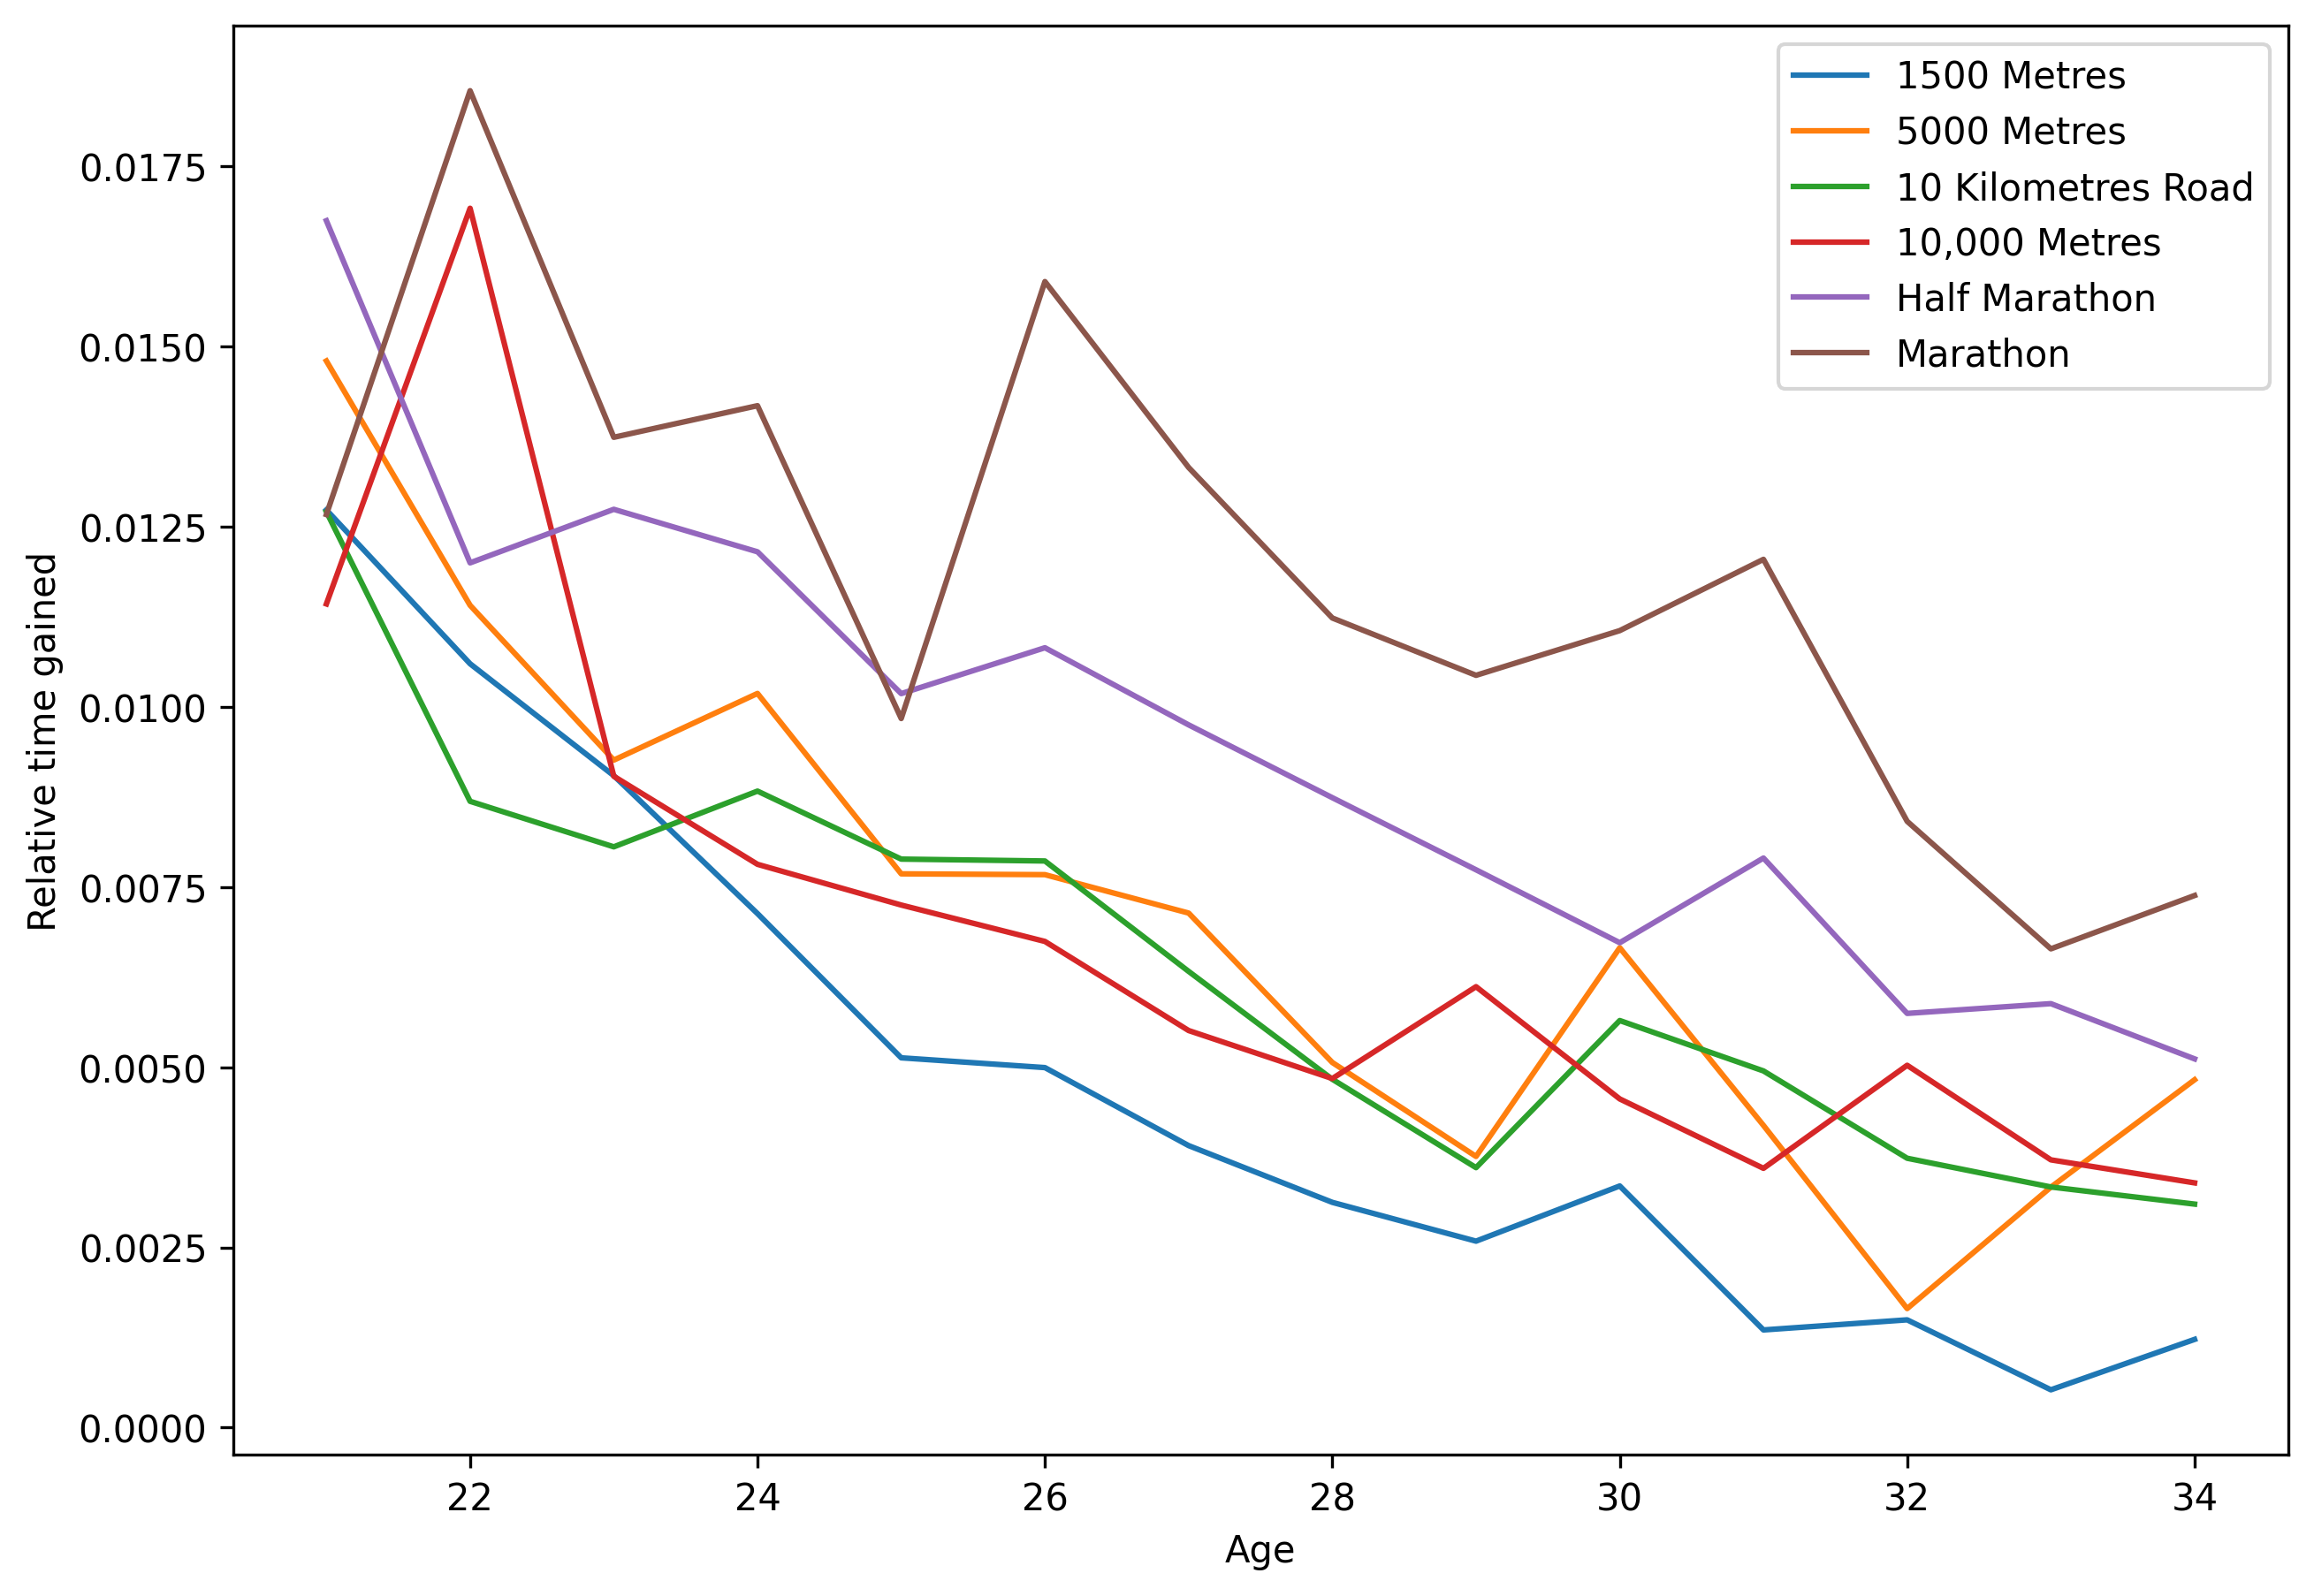
\includegraphics[width=\linewidth]{Data/Figures/Women_Athletes_progression.png}
        \caption{Average progression for women}
        \label{fig:women_progression}
    \end{subfigure}
    \caption{Progression of athletes over time}
    \label{fig:athletes_progression}
\end{figure}

As we could have predicted, the progression decreases with age, as athletes get closer to the limits of human abilities. It is to be noted that the closer they are to that limit, the more significant a time progression is, so a low progression doesn't necessarily translate to "bad" performances. 

The second thing we can notice is that the longer the distance, the bigger the opportunity to improve. There are many factors that can explain that, the main one probably being the fact that the longer the distance, the more parameters there are to optimise : from nutrition before and during the race, to hydration or the race conditions. Another parameter is the fact that an elite athlete that runs in the 1500m can run a competition at peak fitness every other week, while a marathon runner usually doesn't compete more than twice a year, which increases the variance of the performances.

It is also interesting to see that female athletes seem to improve by larger margins during their career compared to men. That could be explained by the fact that running was closed for a long time to women athletes (for reference it was only in 1967 that a woman, Kathrine Switzer, ran the Boston marathon against the rules at the time), so there might be more margins to make progress. \\

\subsection{Athletes clustering}

The idea in this part is to try to characterise an athlete profile using clustering (and PCA for visualisation purposes). For this question, each athlete will be represented by the vector containing all of his best career performance. The challenge here is the fact that most athletes will have NaN in their data, as athletes usually focus on a couple of distances at the same time. 

The first part will be to handle these NaN : as I will be using a KNN model to cluster the data after this steps, it is necessary to impute the data. The technique i used for this task is a KNN imputation (in practice i used the KNNImputer from the sklearn library in Python). This is coherent with the data, as if two persons have similar times on a distance they would probably hit similar times on other distances (it is obviously not as simple as that in reality but with the lack of full data, it is probably the most efficient technique given the dataset). This technique relies on rows where the data is full (there is no NaN in that row). Because there are not many of those rows, the number of neighbors considered for the imputation is quite low, here k=3. The imputed value will then be the mean value of those 3 nearest neighbors.

Once we have got a table full of values, we can proceed to the clustering of the data : each athlete is represented by his full vector of real and/or predicted performances. I then do a cross-validation to tune the number of clusters that fit best to the data, for that I do a grid search of the number clusters between 2 and 7 (we don't want too many clusters as sit will likely overfit and be difficult to interpret) and measure the fit of the data using the average silhouette score. The silhouette score for cluster i is defined as 
\begin{enumerate}
    \item Let \( a(i) \) define $a(i)$ the average distance inside the cluster $i$: 
    \[
    a(i) = \frac{1}{|C_i|-1} \sum_{j \in C_i, i \neq j} d(i, j)
    \]

    \item And $b(i)$ the minmum distance for points outside the clusters
    \[
    b(i) = \min_{k \neq i} \frac{1}{|C_k|} \sum_{j \in C_k} d(i, j)
    \]
    where \( C_k \) is a cluster that does not contain $i$.

    \item The silhouette score for observation $i$, is then defined as:
    \[
    s(i) = \frac{b(i) - a(i)}{\max\{a(i), b(i)\}}
    \]
\end{enumerate}

It measures the separation of the data. In this case the ideal number of clusters is 2 for both the men and the women (it's quite satisfying to have similar results for the two as there are likely to have the behaviour).

After fitting the models, it is obviously difficult to plot a data that is 5 dimensional (6 dimensional if you count the clusters), therefore I am going to use a PCA technique to get the two most relevant features, plot them one against the other to visualise the clusters and try to understand what they mean : for visualisation purposes, I highlighted the names of a few of the best runners in the world, for distances between the 1500m (Jakob Ingebrigtsen who is the best in the world for the 1500m and the 5000m), or specialists of the marathon (like Kelvin Kiptum). Finally, athletes like Kipchoge or Sifan Hassan have some of the best times in numerous events : Sifan Hassan is in the top 10 in world rankings from the 5000m to the marathon (!). I also highlighted 3 random athletes from the second cluster, for reasons that will be explained below.


\begin{figure}[htb]
    \centering
    \begin{subfigure}[b]{0.45\linewidth}
        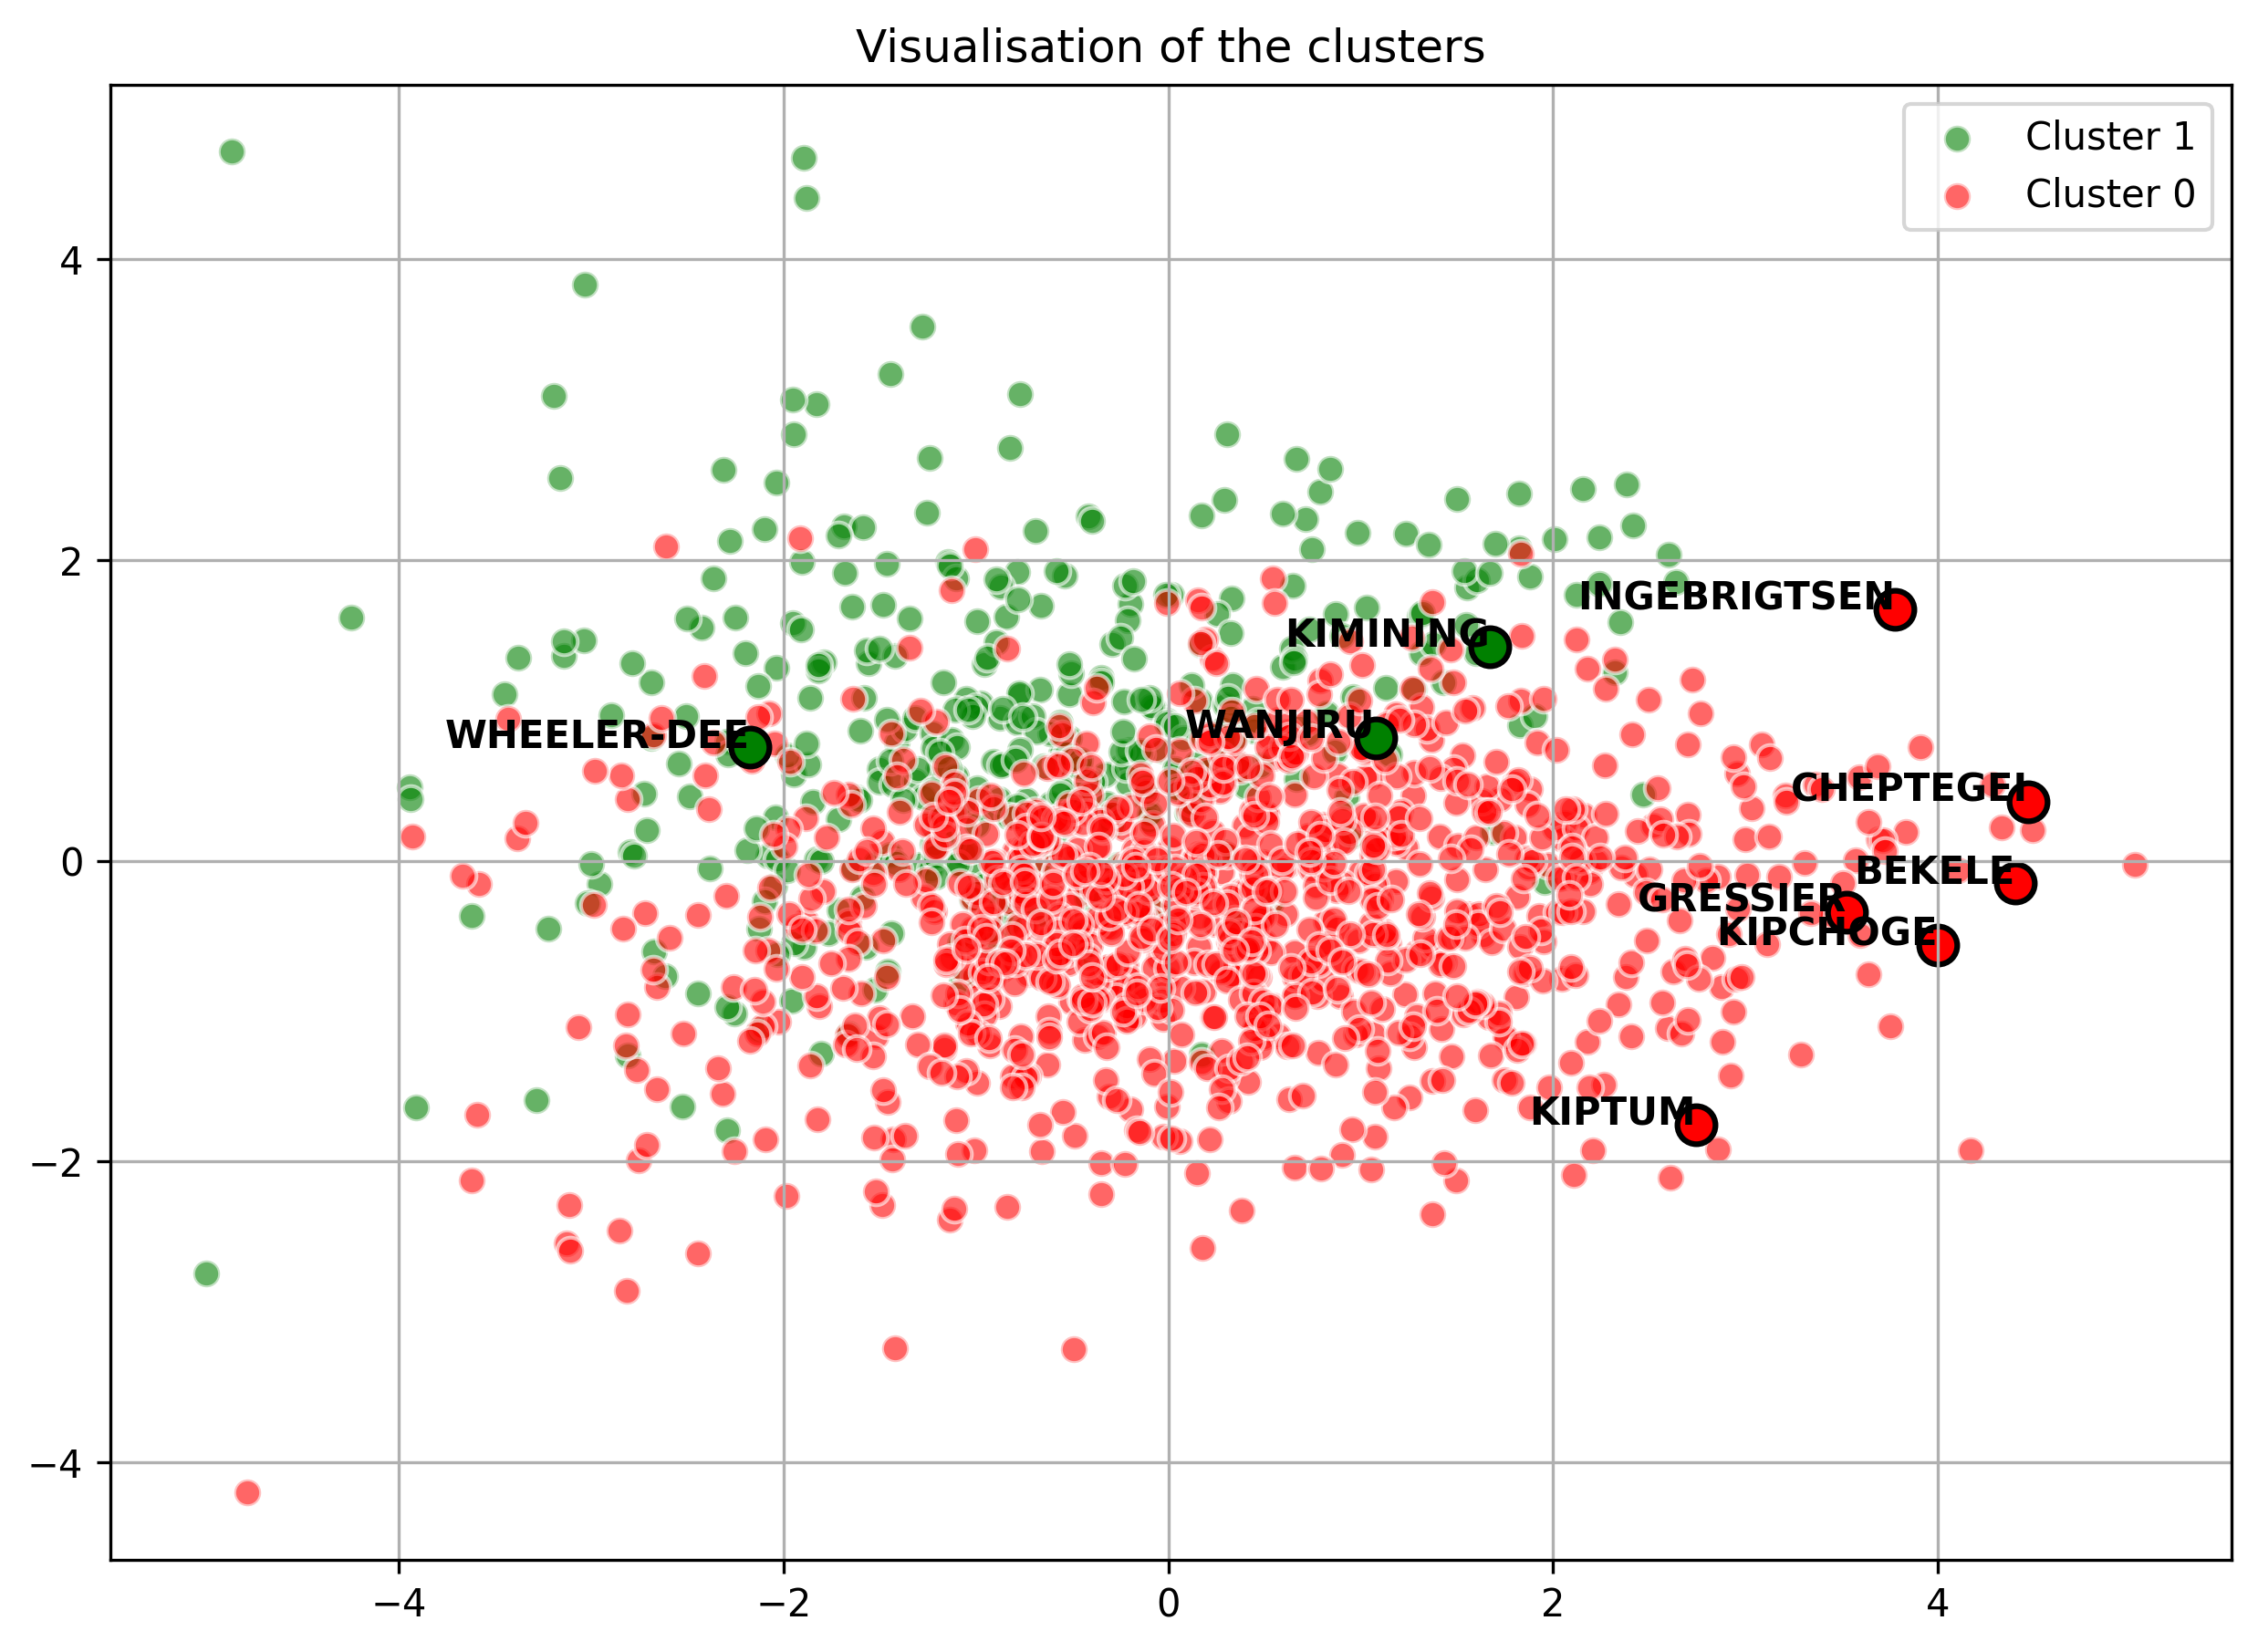
\includegraphics[width=\linewidth]{Data/Figures/Men_Athletes_clustering.png}
        \caption{Men clustering visualisation}
        \label{fig:men-clustering}
    \end{subfigure}
    \hfill
    \begin{subfigure}[b]{0.45\linewidth}
        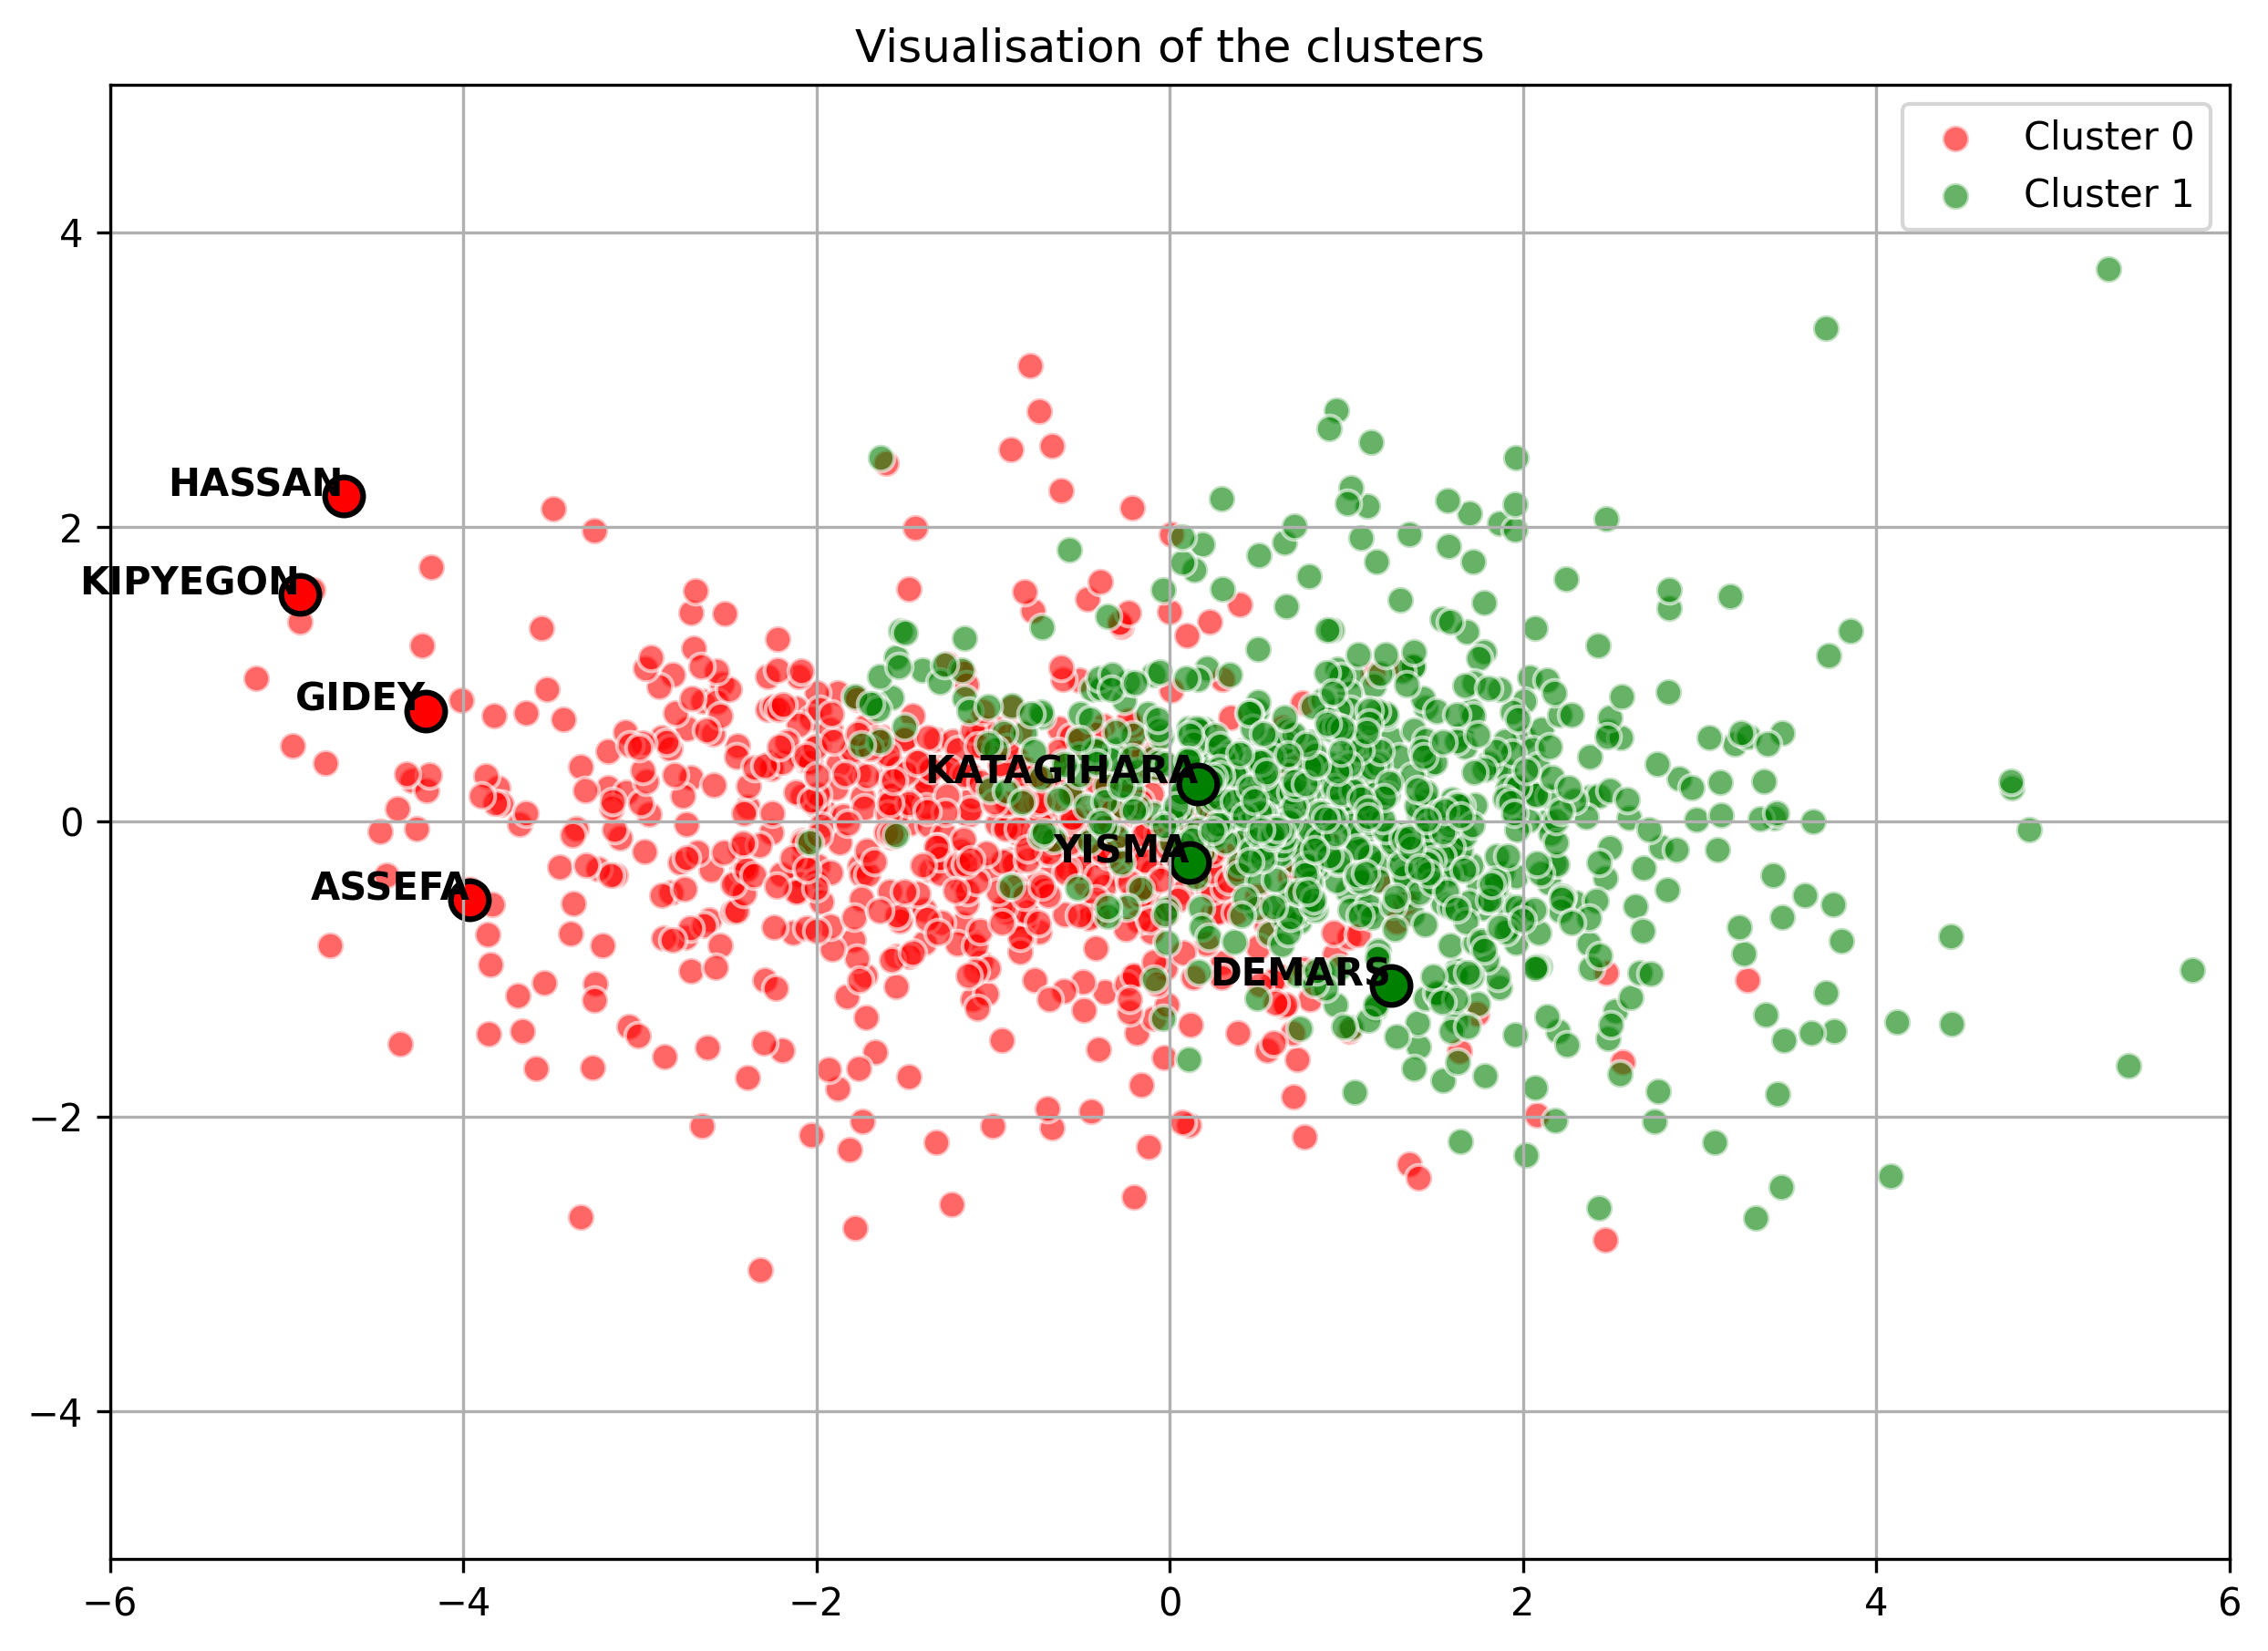
\includegraphics[width=\linewidth]{Data/Figures/Women_Athletes_clustering.png}
        \caption{Women clustering visualisation}
        \label{fig:women-clustering}
    \end{subfigure}
    \caption{Athletes clustering visualisation}
    \label{fig:clustering}
\end{figure}

The result (figure \ref{fig:clustering}) of the clustering leaves me quite surprised as I would have expected something that would look more like endurance (long distances athletes) against the ones that are specialised in shorter distances. On the contrary, it seems that the clustering was more about separating the levels of the athlete, one with the best athletes all distances combined, against the "worst" ones (if that can be said about a top 400 athlete). In the PCA, we can see that the very best athletes are clustered in the same area. Those athletes could almost be considered as outliers and are clearly detached from the rest.
The conclusion of this project is pretty ironic as the data analysis is as ruthless as high level sports : there is a single reality that counts, it is how well you are able to perform.

\end{document}


